\documentclass{article}
\usepackage{graphicx}
\usepackage{hyperref}
\usepackage{float}
\usepackage{longtable}
\usepackage{pgfplotstable}
\usepackage{booktabs} % For better looking tables
\usepackage[utf8]{inputenc}  % Add to preamble

\begin{document}

\begin{titlepage}
% Title and Date - Centered
\centering
{\Huge \underline{\textbf{Assignment 2}}} \\[0.7cm]
{\Large \textbf{Fundamentals of Data Science Lab}} \\[0.5cm]
{\large \textbf{Session: Jan - May 2025}} \\[0.5cm]  % Automatically inserts the current date
{\large Programme: BTech. CS - Data Science} \\[0.5cm]  % Automatically inserts the current date
{\large Sem: 4} \\  % Automatically inserts the current date
{\large Batch: 5}  % Automatically inserts the current date

\vfill
% Author and Professor Name in Separate Columns
\begin{center}
      \begin{minipage}[t][3cm][t]{0.45\textwidth}  % Same fixed height, top alignment
        \textbf{Submitted By:} \\[0.15cm]
        Name: Kshitij Chandrakar \\
        SAP ID: 500124827
    \end{minipage}
    \hfill
      \begin{minipage}[t][3cm][t]{0.45\textwidth}  % Same fixed height, top alignment
        \raggedleft  % Right-aligns text
        \textbf{Submitted To:} \\[0.15cm]
        Dr. Sachi Chaudhary
    \end{minipage}
\end{center}
\end{titlepage}


\section{Dataset Information}\label{dataset-information}

\paragraph{Dataset Chosen:}
 APOGEE2 from SDSS\\
\url{https://www.sdss4.org/dr17/irspec/spectro_data}
\paragraph{Objective:}
Identifying Stars from the Halo of Our Galaxy Based on Various Stellar Parameters\\
\paragraph{Description and Selection Process}
We choose the dataset as it has good support with multiple Value Added Catalogs, Was released  relatively recently so it would have more accurate Information, it is Well Documented and has Features which would help our Objective.\\
It is a part of The Sloan Digital Sky Survey. They have created the most detailed three-dimensional maps of the Universe ever made, with deep multi-color images of one third of the sky, and spectra for more than three million astronomical objects.
\paragraph{Hypothesis}
From the current theory, we can Hypothesise that the Halo stars would have the following properties.
\begin{itemize}
  \item Spatial Distribution with an angled Galactic Latitude
  \item Metal Poor \([Fe/H] < −1\)
  \item Highly Turbulent Motion
  \item Highly eccentric and inclined orbits
  \item alpha-element enhancement (O, Mg, Si)

\end{itemize}
% =========================================
% =========================================
% =========================================
\newpage
\section{Exploratory Data Analysis} On doing EDA we find various trends, the
following are the Observations.\\
% =========================================
\subsection{Data Density and Galactic Coordinates}
\begin{figure}[H]
   \centering
   \label{fig:1}
   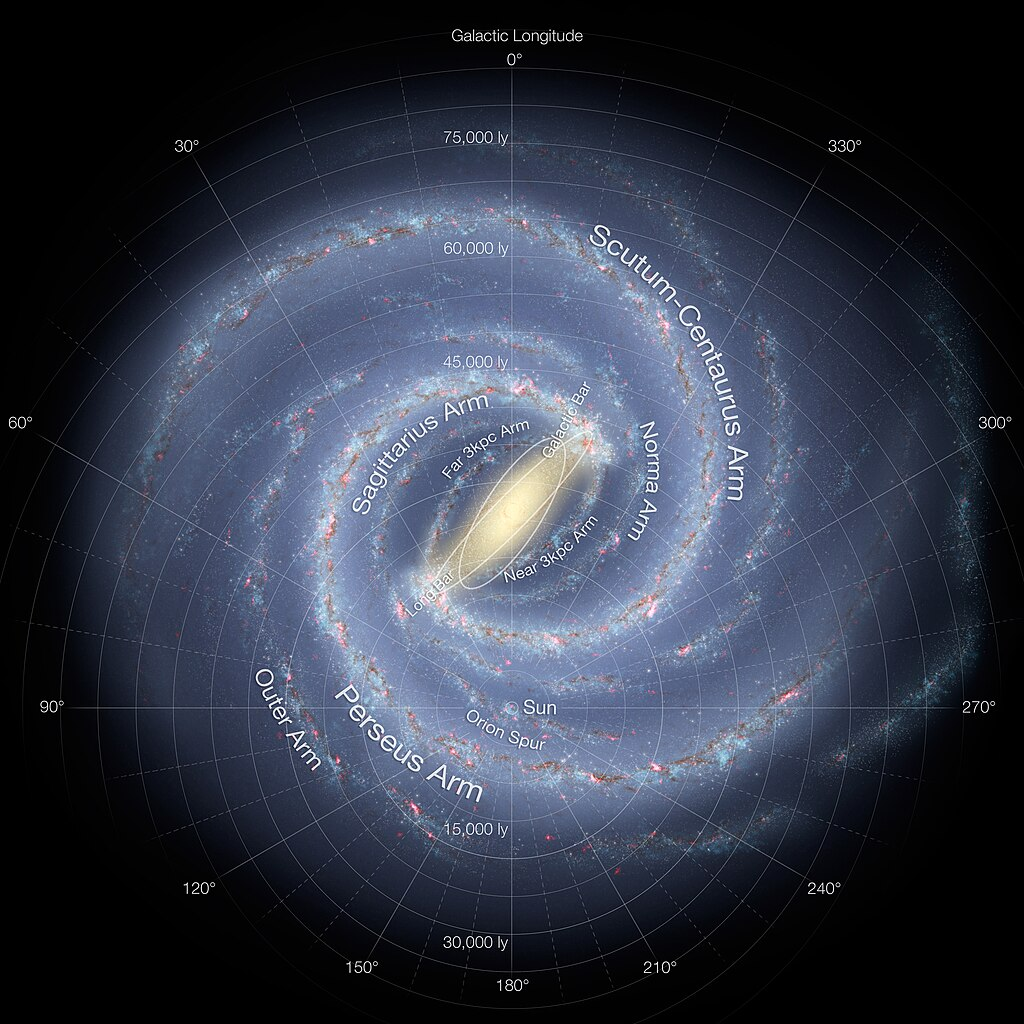
\includegraphics[width=\textwidth]{Images/GalacticCoordinates.jpg}
   \caption{Galactic Coordinate System}
\end{figure}

\paragraph{}
The \hyperref[fig:1]{Artist's depiction} Above of the Milky Way Galaxy showing the origin and orientation of galactic longitude. The galactic longitude (l) runs from the Sun upwards in the image through the center of the galaxy. The galactic latitude (b) is perpendicular to the image (i.e. coming out of the image) and also centered on the Sun.

\paragraph{}
From a the \hyperref[fig:2]{APOGEE Targetting Field Map} and \hyperref[fig:3]{Density plot} of the data points we can see that the data is slighly biased as we physically cannot observe the stars on the opposite side of our galaxy. However, the stars we can observe are well recorded. with only a few peaks in the interesting regions like the Magellanic Clouds.

\begin{figure}[H]
   \centering
   \label{fig:2}
   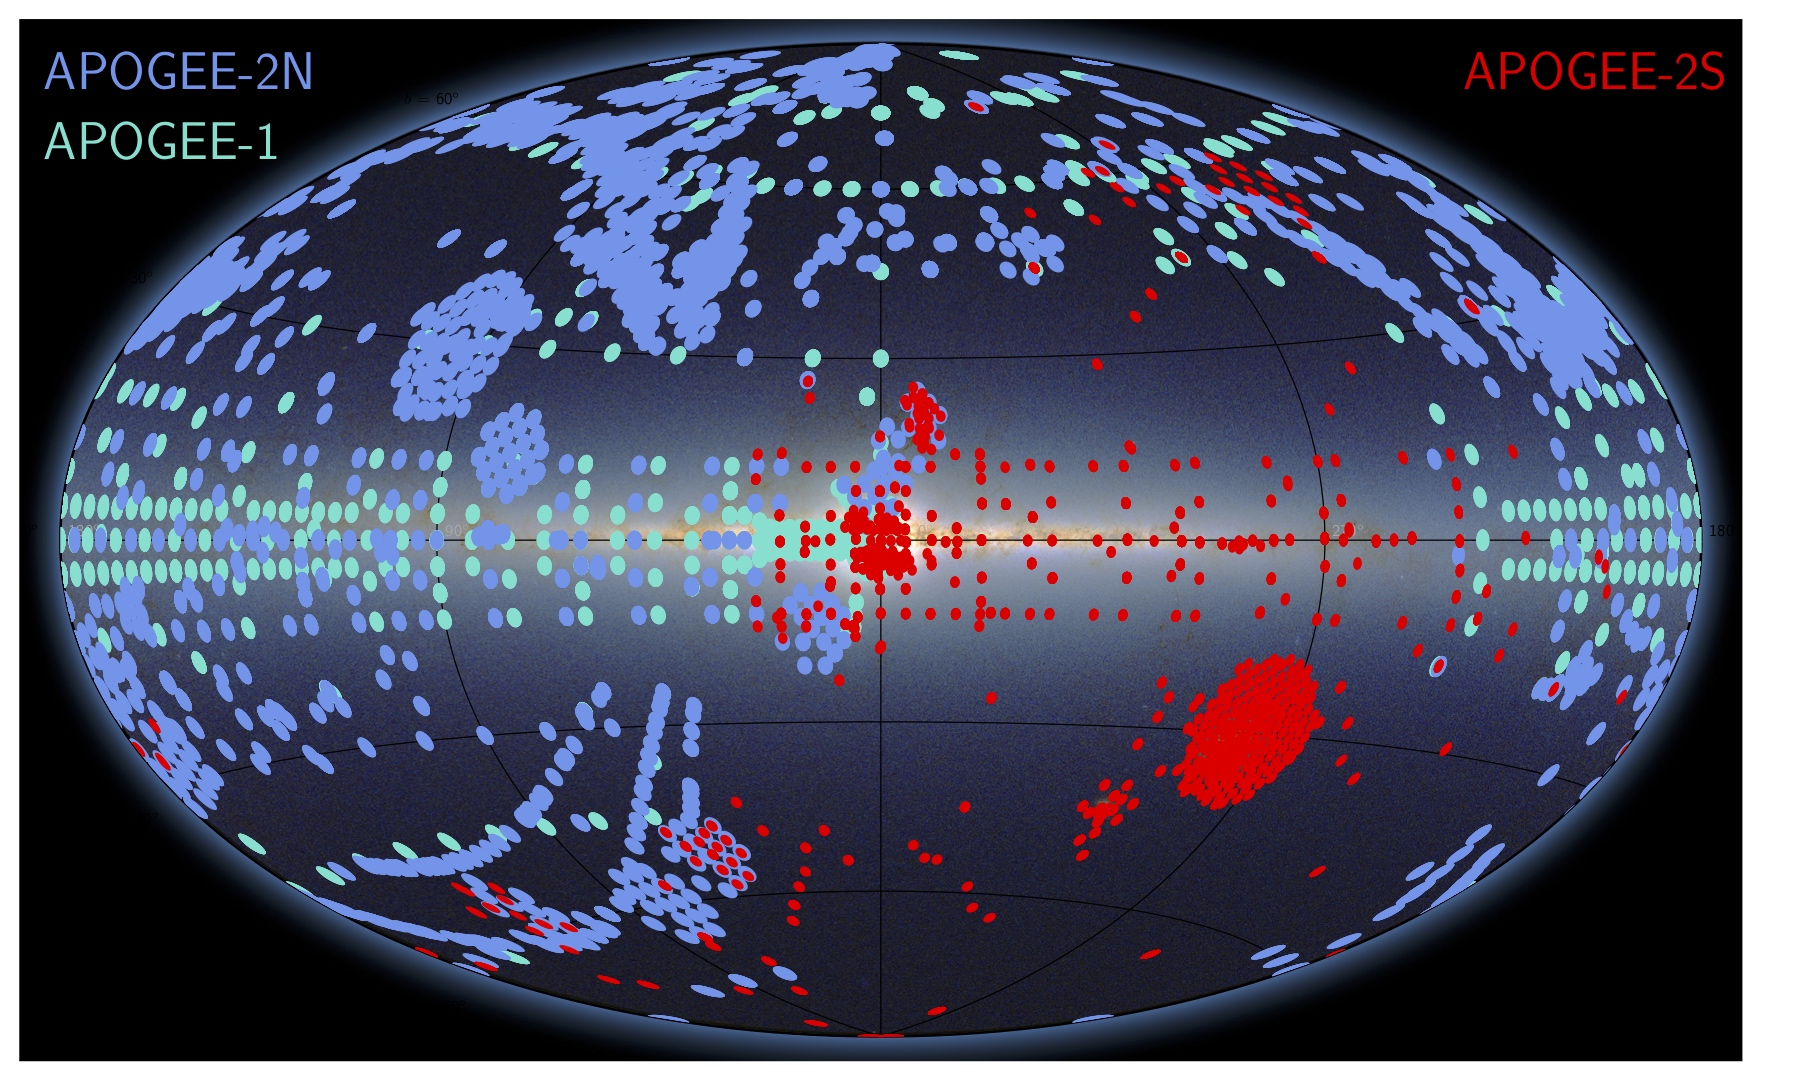
\includegraphics[width=\textwidth]{Images/ApogeeCoverage.jpg}
   \caption{DR17 APOGEE field map where the fields are color-coded by the APOGEE sub-survey. APOGEE-1 in cyan, APOGEE-2N in blue, and APOGEE-2S in red. Figure by C. Hayes. Background image from 2MASS.}
\end{figure}
\begin{figure}[H]
    \centering
    \label{fig:3}
    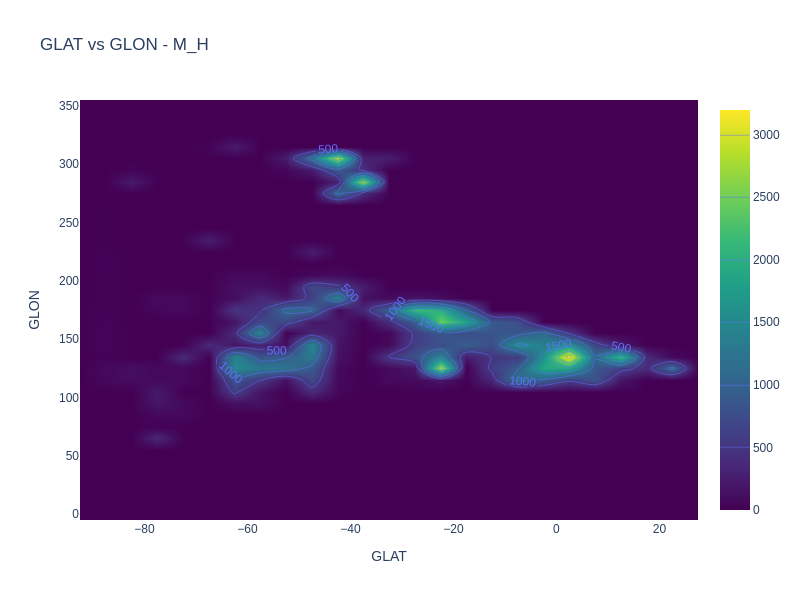
\includegraphics[width=\textwidth]{Images/GLAT vs GLON - Density.png}
    \caption{Density Plot}
\end{figure}

% =========================================
\subsection{HR Diagram}
\begin{figure}[H]
    \centering
    \label{fig:4}
    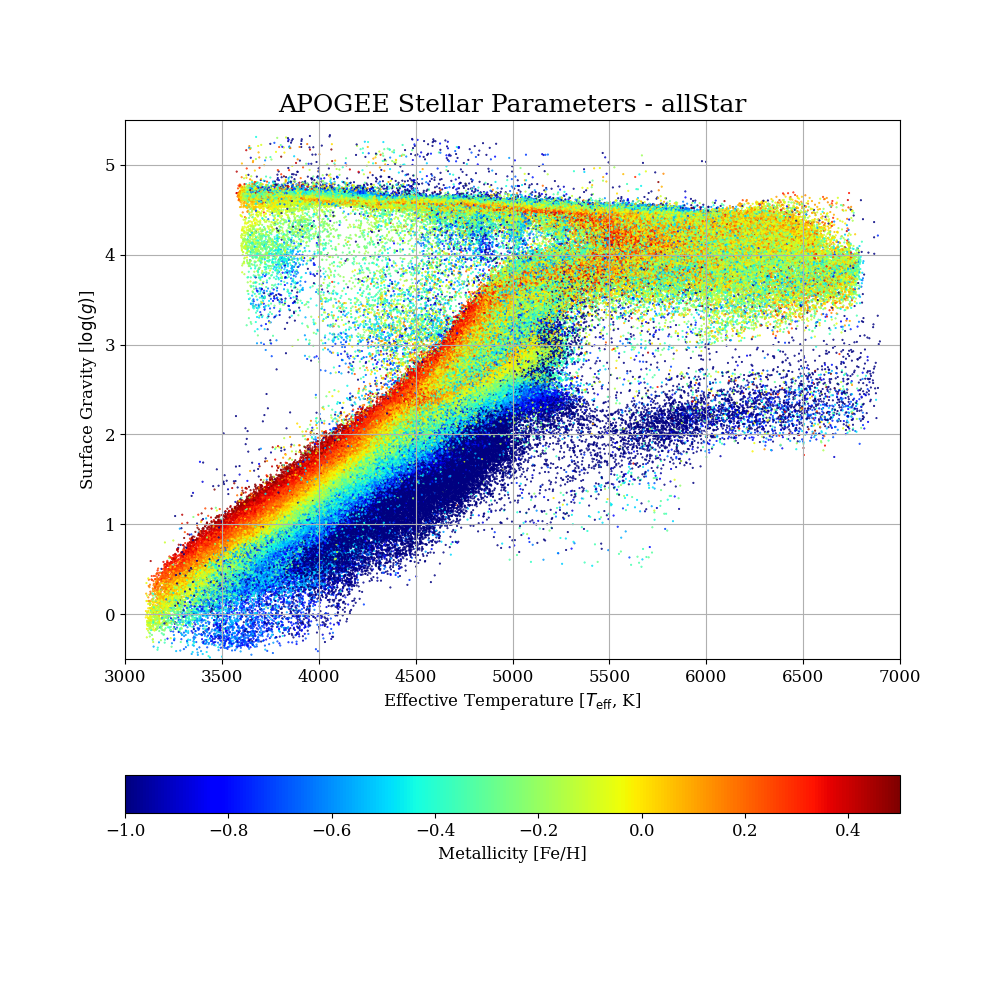
\includegraphics[width=\textwidth]{Images/APOGEEStellarParameters-allStar.png}
    \caption{HR - Diagram}
\end{figure}
From a \hyperref[fig:4]{scatterplot} between  Effective Temperature at Surface \(T_{eff}\) and the Surface Gravity \(log( g)\) we can see that:
\begin{itemize}
  \item the Relationship is mostly linear upto \(T_{eff} < 5000K\) and \(log(g) < 3\), this is known as the main sequence of stars, which is most of the lifetime of the star. Any given star moves from a lower Metallicity to a Higher Metallicity as it grows Older.

  \item The star moves above \(T_{eff} > 5000K\) and \(log(g) > 3\) when its dying, converting to various types of Dead Stars such as Red Giants, Red Supergiants, White Dwarfs, Neutron Stars and Black holes depending on a mixture of various variables.
\end{itemize}
% =========================================
\subsection{Star Formation Regions}
\begin{figure}[H]
    \centering
    \label{fig:5}
    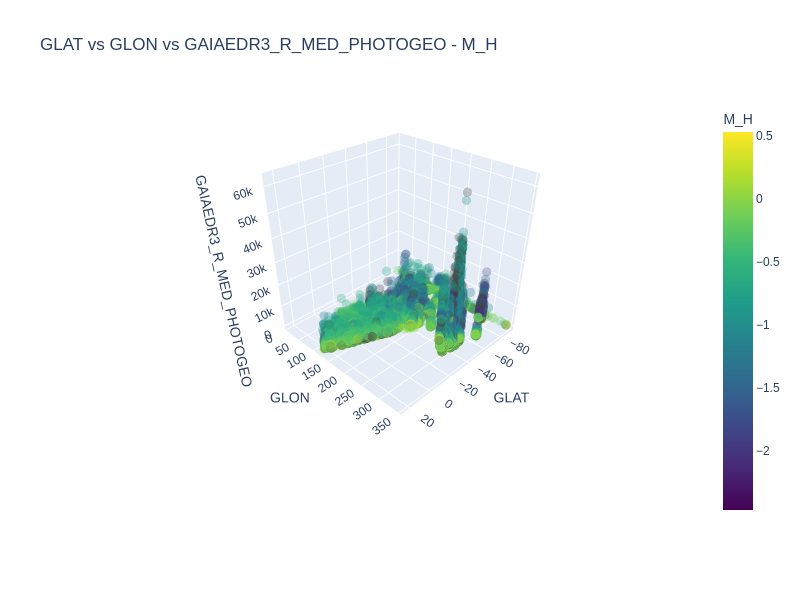
\includegraphics[width=\textwidth]{Images/GLAT vs GLON vs Distance - M_H.png}
    \caption{GLAT vs GLON vs Distance Colored by M_H}
\end{figure}
\paragraph{}
In the above \hyperref[fig:3]{Scatterplot} we can Identify the various regions with a high star formation rate. They can be identified by the clumps of datapoints which are a deep blue.
\paragraph{}
The Deep-Blue Signifies a Low Metallicity which means that the particular star is Young.
% =========================================
\newpage
\section{Feature Selection}\label{feature-selection}

Techniques Applied:
\begin{itemize}
  \item Correlation Matrix
  \item Random Forest Selection
  \item Lasso Regression
\end{itemize}

% =========================================
\subsection{Correlation Matrix}
We create the Covariance Matrix Heatmap and Remove Highly Correlated Features with \( | r |  > 0.85 \):\\

\begin{figure}[H]
    \centering
    \label{fig:6}
    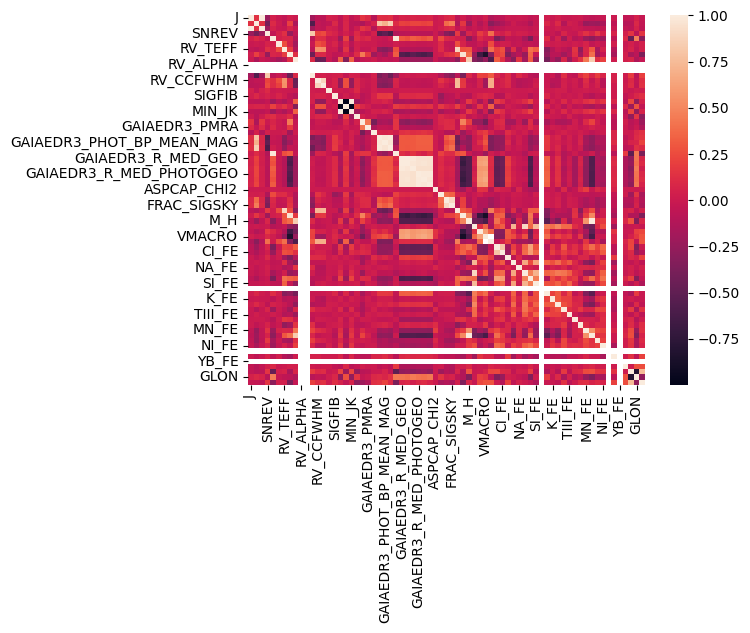
\includegraphics[width=\textwidth]{Images/CorrelationMatrixBetweenNumerical1.png}
    \caption{HR - Diagram}
\end{figure}


After Dropping we get the following columns left:
\paragraph{}
`J', `H', `K',
`SNREV', `VHELIO\_AVG', `VSCATTER', `RV\_TEFF', `RV\_LOGG', `RV\_FEH', `RV\_ALPHA', `RV\_CARB', `RV\_CHI2', `RV\_CCFWHM', `RV\_AUTOFWHM', `MEANFIB', `SIGFIB', `MIN\_H', `MAX\_H', `MIN\_JK', `MAX\_JK', `GAIAEDR3\_PARALLAX', `GAIAEDR3\_PMRA', `GAIAEDR3\_PMDEC', `GAIAEDR3\_PHOT\_G\_MEAN\_MAG', `GAIAEDR3\_PHOT\_BP\_MEAN\_MAG', `GAIAEDR3\_PHOT\_RP\_MEAN\_MAG', `GAIAEDR3\_DR2\_RADIAL\_VELOCITY', `GAIAEDR3\_R\_MED\_GEO', `GAIAEDR3\_R\_LO\_GEO', `GAIAEDR3\_R\_HI\_GEO', `GAIAEDR3\_R\_MED\_PHOTOGEO', `GAIAEDR3\_R\_LO\_PHOTOGEO', `GAIAEDR3\_R\_HI\_PHOTOGEO', `ASPCAP\_CHI2', `FRAC\_BADPIX', `FRAC\_LOWSNR', `FRAC\_SIGSKY', `TEFF', `LOGG', `M\_H', `ALPHA\_M', `VMICRO', `VMACRO', `VSINI', `C\_FE', `CI\_FE', `N\_FE', `O\_FE', `NA\_FE', `MG\_FE', `AL\_FE', `SI\_FE', `P\_FE', `S\_FE', `K\_FE', `CA\_FE', `TI\_FE', `TIII\_FE', `V\_FE', `CR\_FE', `MN\_FE', `FE\_H', `CO\_FE', `NI\_FE', `CU\_FE', `CE\_FE', `YB\_FE', `RA', `DEC', `GLON', `GLAT'
% =========================================
\subsection{Lasso L1 Regression}
We do Lasso Regression with \(\alpha=0.1\) and get the following features with Non-Zero Coefficients. We do not expect this to be accurate as L1 regression is not accurate for non linear data.
\paragraph{}

\pgfplotstabletypeset[
  col sep=comma,
  string type,
  every head row/.style={
    before row=\toprule,
    after row=\midrule
  },
  every last row/.style={
    after row=\bottomrule
  }
]{Data/Lasso.csv}

% =========================================
\subsection{Random Forest}
We do a Random Forest Feature selection with \(n_estimators=100 and random_state=42\) and get the following features. We expect this method to give us a more accurate result of what features are the most important as it works well with multivariant and non-linear data.
\paragraph{}
we can see that the most important features are GLAT, VMACRO, M/H, F/H, N/FE and VSCATTER; which tracks with our objective of mapping Halo stars.
\paragraph{}

\pgfplotstabletypeset[
  col sep=comma,
  string replace*={_}{\textunderscore},
  begin table=\begin{longtable},
  end table=\end{longtable},
  every head row/.style={
    before row={\toprule
                Feature & Importance \\
                \midrule},
    after row={\endhead
               \bottomrule\endfoot},
  },
  columns={Feature,Importance},
  columns/Feature/.style={string type, column type=l},
  columns/Importance/.style={column type=r, fixed, precision=6},
]{Data/RandomForest.csv}
\section{Conclusion}
In Conclusion, We can see that the various stellar parameters selected by the Various Techniques reflect their own Advantages and Disadvantages, with the Random Forest Being the most accurate and suitable for our dataset. It selected the most accurate and applicable Features to fit our Hypothesis.
\end{document}
